\documentclass[a4paper,12pt]{article}
\usepackage{caption}
\usepackage{subcaption}
\usepackage{float}
\usepackage[T1]{fontenc}
\usepackage[italian]{babel}
\usepackage[utf8]{inputenc}
\input funzioni.sty
\input funzioni2.sty
\floatstyle{ruled}
\usepackage{hyperref}
\usepackage{graphicx}
\usepackage{amsmath}
\usepackage{amssymb}
\usepackage[width=125mm]{caption}
\usepackage{amsthm}
\usepackage{algorithm2e}
% Dimensione della pagina
\setlength{\oddsidemargin}{.3in}  % Distance from the left edge -1 inch 
\setlength{\textwidth}{145mm}     % Normal width of the text
\setlength{\topmargin}{.25in}     % Distance from top to PAGE'S HEAD -1 inch
\setlength{\textheight}{225mm}    % Height of the body of page
\setlength{\headheight}{0mm}      % Height of a box containing the head
\setlength{\parskip}{0.5mm}         % Extra vertical space before a paragraph
\setlength{\parindent}{9mm}       % Width of the indentation 
\linespread{1.12}                 % Line spacing        
\renewcommand{\floatpagefraction}{.9}

\begin{document}
\author{Stefano Mandelli}
\title{\bf \Huge Confronto delle prestazioni CPU-GPU per la simulazione di un reticolo di Ising-2D}
\date{}
\maketitle
\section*{Introduzione}
Per confrontare le prestazioni di CPU e GPU in questo lavoro è stato scelto il modello di Ising 2D. \`E un modello analitico, nel senso che al limite termodinaco esiste una soluzione analitica esatta. E' stato possibile riportare il codice, operazione per operazione (compresa la generazione dei numeri pseudorandom) da singola CPU all fine parallelizzazione delle GPU, in questo modo sarà possibile valutare lo speed-up di prestazioni in modo quantitativo perfettamente consistente. Se si fosse usato un generatore di numeri pseudorandom diverso, la comparazione sarebbe stata meno consistente in quanto si sarebbero andati a comparare risultati ottenuti con implementazioni diverse. I punti che verranno trattati in questo lavoro sono i seguenti:
\begin{itemize}
	\item Breve introduzione sul modello usato;
	\item Implementazione del codice;
	\item Consistenza fisica del modello;
	\item Discussione suulla diversità dei risultati;
	\item Comparazione delle prestazioni per diverse implementazioni;
\end{itemize}

\section{Scelta del modello}
Il modello di Ising-2D è un modello che si presta molto bene ad essere parallelizzato, in quanto è un tipico modello interagente a corto range. In questo modo è possibile pensare ad una strategia di parallelizzazione efficace. Brevemente, il modello di Ising è caratterizzato da un reticolo (ad esempio ipercubico) in $D$ dimensioni. Ad ogni cella del reticolo viene associato uno spin si che può essere solo del tipo $s_i=\lbrace +1, -1 \rbrace$ a seconda che la direzione del dipolo magnetico (o spira), associato alla cella $i-esima$ del reticolo risulti verso l'alto o verso il basso. Il sistema è descritto dall’Hamiltoniana di Ising
\newl{\mathcal{H}=-J\sum_{\langle i,j\rangle}s_is_j -h\sum_{i}s_i}
dove $h$ identifica un eventuale campo magnetico uniforme esterno. La prima sommatoria è fatta su tutte le coppie di siti primi vicini e $J$ indica la costante di accoppiamento tra spin. In questo lavoro si considera il caso il caso $D = 2$ dimensionale, $J > 0$ e campo magnetico esterno nullo, quindi $h = 0$. Al limite termodinamico, il modello di Ising (escluso il caso $1D$) presenta una transizione di fase in prossimità di una temperatura critica $T_c$ . Per temperature maggiori di $T_c$ il sistema si comporta in modo paramagnetico. Per temperature inferiori invece si ha un fenomeno di magnetizzazione spontanea. Le principali grandezze fisiche che possono essere calcolate sono la magnetizzazione media del sistema $\langle M\rangle$  e la capacità termica a volume costante $\langle C_V \rangle$ che viene calcolata col teorema di fluttuazione-dissipazione. Tutte queste quantità estensive sono divergenti nel limite termodinamico. Nelle simulazioni statistiche vengono considerati dei modelli finiti di $N = D \times D$ spins che si desidera confrontare per diversi size. È utile pertanto confrontare la densità di energia $e = E /N$, la densità di calore specifico $c_V = CV /N$ e di magnetizzazione che è la variabile coniugata al campo esterno $h$
\newl{m=\frac{1}{N}\langle\sum_is_i\rangle}
Per il caso $h = 0$ e $T > T_c$ , $\langle M \rangle$ si annulla. Questo comportamento può essere spiegato nel seguente modo: per $T > T_c$ le fluttuazioni termiche prevalgono sulla tendenza del termine di interazione $J$. La lunghezza di correlazione è molto piccola e ogni spin ha la stessa probabilità di avere come valore $+1$ o $-1$, in questo modo $\langle M \rangle$ risulta nulla. Per temperature $T < T_c$ gli spin risentono fortemente dell’interazione coi loro primi vicini. Si nota che in questo range di temperature il modello di Ising 2D, presenta una transizione di fase netta. Il sistema passa, in modo spontaneo, da una situazione di ordine in cui gli spin sono orientati prevalentemente nella stessa direzione quindi hanno in maggioranza valore $+1$ oppure $-1$. I due casi, per campo magnetico esterno nullo $(h = 0)$, sono equiprobabili, in quanto per $h = 0$ l’Hamiltoniana di Ising è pari per inversione di tutti gli spins, per tempi molto lunghi entrambi gli stati vengono popolati per la stessa quantità di tempo facendo risultare, anche in questo caso, $m = 0$. Per modelli finiti sufficientemente grandi è ugualmente possibile effettuare delle valutazioni e misure di magnetizzazione media spontanea del sistema per $T < T_c$ . Questo si ottiene settando lo stato di partenza in modo tale che uno dei due stati sia più popolato dell’altro. Se per convenzione si sceglie uno stato di partenza con una maggioranza di spins a valore $+1$, lo stato di equilibrio dell’Hamiltoniana di Ising, con molti spin a valore $+1$ sarà favorito. In questo modo, per temperature inferiori a quella critica, si hanno dei valori di magnetizzazione non nulli e dello stesso segno ed è quindi possibile valutare l’entità della magnetizzazione spontanea.
\subsection{Algoritmo di Metropolis}
Dato che le fluttuazioni di energia, rispetto all'energia totale del sistema, sono piccole, un modo sufficientemente efficiente di generare delle mosse Monte Carlo, è quello definito dalla \textit{dinamica a singolo spin-flip}. I vari stati vengono generati in modo che il successivo sia differente dal precedente per il flip di un singolo spin del reticolo preso inizialmente in modo casuale. Lo stato $\mu$ e quello $\nu$ differiscono tra loro solo per il flip di un singolo spin. In questo modo è possibile definire la probabilità di selezione come
\newl{g(\mu\to\nu)=\frac{1}{N}\,.}
Con questa probabilità di selezione, la condizione del detailed balance prende la forma
\newl{\frac{P(\mu\to\nu)}{P(\nu\to\mu)} = \frac{g(\mu\to\nu)A(\mu\to\nu)}{g(\nu\to\mu)A(\nu\to\mu)} = \frac{p_\nu}{p_\mu} = e^{-\beta (E_\nu-E_\mu)}\,. \label{DET:FIN} }
Dato che $g(\mu\to\nu)=g(\nu\to\mu)$ si sceglie l'acceptance ratio in modo tale che soddisfi l'equazione $(\ref{DET:FIN})$
\newl{\frac{A(\mu\to\nu)}{A(\nu\to\mu)} = e^{-\beta (E_\nu - E_\mu)},}
da cui è possibile dedurre che
\newl{A(\mu\to\nu) = A_0 e^{-\frac{1}{2}\beta(E_\nu-E_\mu)}\label{acc-rat-azer}\,.}
Per avere un algoritmo che sia il più efficiente possibile l'acceptance ratio deve essere significativamente diversa da zero. Il parametro $A_0$ è scelto in funzione ad alcune considerazioni
su come è fatta l'Hamiltoniana di Ising. E' facile osservare che la differenza di energia tra due stati, in modulo, è al massimo pari a $|\Delta E|=2zJ$ dove $z$ è il numero di primi vicini, che nel
caso di reticolo 2D vale $z=4$, quindi per il reticolo 2D abbiamo che al massimo $|\Delta E|= 8J$. La differenza di energia tra lo stato $\mu$ e $\nu$ è
\newl{|E_\nu-E_\mu| \leq 2zJ.}
In questo modo, il massimo possibile valore dell'esponenziale vale
\newl{e^{-\frac{1}{2}\beta (E_\nu-E_\mu)} \leq e^{\beta zJ}}
che permette di stabilire la scelta migliore possibile del coefficiente
\newl{A_0 = e^{-\beta zJ}\,.}
La scrittura finale per l'acceptance ratio risulta quindi:
\newl{A(\mu\to\nu)= e^{-\frac{1}{2} \beta(E_\nu-E_\mu + 2zJ) },\label{acc:ratio}}
in modo da avere $A(\mu\to\nu) \leq 1$.
Si può verificare che l' $A(\mu\to\nu)$ scritta ora è molto inefficiente. Il sistema rimane per troppo tempo nello stesso stato. Una scelta migliore che rispetta tutte le condizioni di quella precedente è data proprio dall'acceptance ratio proposta da Metropolis
\begin{equation} 
A(\mu\to\nu)=\left\{
        \begin{aligned}
                \label{acc2:ratio}
                &e^{-\beta(E_\nu-E_\mu)} &E_\nu-E_\mu > 0 \\
                &1 &\text{altrimenti.}
        \end{aligned}
        \right.
\end{equation}
Per il modello di Ising le acceptance ratio appena descritte hanno la particolarità che possono essere calcolate mediante la sola conoscenza degli spins primi vicini allo spin di cui si propone il suo flip, questo perchè l'interazione nel modello di Ising  è a corto raggio. Nel caso dell'Hamiltoniana di Ising, questa differenza è possibile scriverla in modo molto semplice, in funzione solo dagli spin primi vicini dello spin di cui si propone il flip:
\newl{
	E_\nu - E_\mu &=& -J\sum_{\langle i,j \rangle}s_i^\nu s_j^\nu + J\sum_{\langle i,j \rangle}s_i^\mu s_j^\mu = \nonumber\\
	&=& -J\sum_{i\neq k}s_i^\nu(s_k^\nu-s_k^\mu) = -2Js_k^\mu\sum_{i\neq k} s_i^\mu\,.
	\label{DIF:EN:SPIN}
}



\section{Implementazione del codice}
L'implementazione del codice passa attraverso due grandi fasi. La prima fase consiste nell'organizzare il reticolo di Ising sulla GPU. L'obiettivo che ci si pone è quello di usare nel modo migliore le aree di memorie in modo da garantire sempre coalescenza, velocità di lettura/scrittura e minimizzazione di banck conflict. La coalescenza consiste nell'effettuare chiamate ad aree di memoria allineate in modo da massimizzare le performance. La velocità di lettura e scrittura dipende dal tipo di memoria usata mente il problema del banck conflict consiste nel fatto che due aree di memoria non possono essere lette contemporaneamente. Se nel programma ci sono chiamate di questo tipo,  vengono schedulate in modo sequenziale perdendo tutto il vantaggio della parallelizzazione.

Una seconda fase consiste nel riportare, operazione per operazione, il generatore di numeri pseudorandom usato nel caso per CPU in parallelo su GPU. Questo tipo di passaggio non è banale in quanto la generazione di numeri pseudorandom è per definizione seriale. La generazione del numero $n+1$ dipende dal numero $n$. Dato che l'evoluzione del nostro modello è di tipo Metropolis e i numeri random sono quindi una necessità assoluta, per non perdere paralelizzazione del codice, è necessario elaborare una strategia di generazione dei numeri pseudorandom parallela e performante per le GPU.

\subsection{Implementazione del modello}
Il reticolo di Ising è stato posizionato sulla griglia  della GPU in due modi differenti. La prima volta usando solo la memoria globale, la seconda volta usando anche quella shared per comparare eventuali migliorie nella performance. Come da equazioni [\ref{DIF:EN:SPIN}] e [\ref{DET:FIN}] l'evoluzione di uno spin dipende solo dai suoi 4 primi vicini. Questo fa sì che la miglior strategia di parallelizzazione sia quella di effettuare gli update del reticolo a scacchiera. Aggiornando prima gli spin "pari" e successivamente quelli "dispari" si vanno ad aggiornare elementi totalmente indipendenti del sistema.

Un secondo livello di gestione del reticolo, è quello di utiilizzare la memoria shared, nota per essere molto veloce in lettura e scrittura. La memoria shared però è divisa in blocchi indipendenti tra loro, questo fa si che il reticolo iniziale, debba essere prima posizionato nella memoria shared, successivamente vanno insierite le condizioni di raccorto blocco/blocco e quindi effettuare l'update degli spin usando una doppia scacchiera, a blocchi grandi (relativi ai blocchi della shared memory) e a blocchi piccoli nel senso dell'update a scacchiera anche dei threads all'interno dello stesso blocco che condividono la stessa area di memoria shared. In Figura \ref{figura:time} sono stati plottati il tempo per proporre un update in funzione al size del reticolo.



\subsection{Implementazione del PRNG}
Una classe di generatori efficienti è stata proposta da Marsaglia ed è quella dei generatori \textbf{xorshift}. Consistono nel scegliere in modo opportuno, un vettore di semi iniziali in cui le componenti sono bits. Se si sceglie un vettore $x$ di lunghezza $w$, è possibile dimostrare che si ottiene un ottimo e molto veloce generatore di numeri pseudo-random effettuando su questo vettore operazioni di shift. Definiamo la matrice $\mathbf{L}$
\newl{
	\mathbf{L}=\left(\begin{matrix}
	0 & 0 & \cdots & 0 \\
	1 & 0 & \cdots & 0 \\
	\vdots & \ddots & \ddots & \vdots\\
	0 & \cdots & 1 & 0
	\end{matrix}\right)
}
come matrice di \textit{spostamento a sinistra} che trasforma il vettore $x=(x_1,\cdots,x_w)$ in $x=(x_2,\cdots,x_w,0)$. L'operazione totale di XORShift proposta da Marsaglia è però di or esclusivo quindi per effettuare uno xorshift di $a$ posizioni si ha che
\newl{
		x_{n+1} = x_{n}(\text{Id}\oplus \mathbf{L}^a ).
	\label{xor:sh}
}
Con il simbolo $\oplus$ si intende la somma con mod $2$ su ogni singolo elemento. Un vettore del tipo $x_{n}=(1,1,0,1)$ viene trasformato con uno xorshift sinistro di $a=1$ nel vettore $x_{n+1}$ diventando
\newl{
		x_{n+1} = x_{n}(\text{Id}\oplus \mathbf{L}^1) = (1,1,0,1)\left(\begin{matrix}
			        1 & 0 & 0 & 0 \\
			        1 & 1 & 0 & 0 \\
			        0 & 1 & 1 & 0\\
			        0 & 0 & 1 & 1
				\end{matrix}\right) = (0,1,1,1).
}
Questa operazione, per quanto riguarda il linguaggio di programmazione C, può essere semplicemente svolta tramite due operazioni di bitwise. Dal punto di vista del codice, 
l'equazione $(\ref{xor:sh})$ risulta molto semplice \texttt{x\;=\;x\;\^\;(x<<a)}. In letteratura viene consigliato di usare quattro step di shift. L'algoritmo implementato è quindi 
\newl{
		x_{n+1} = x_n(\text{Id}\oplus \mathbf{L}^a) (\text{Id}\oplus \mathbf{R}^b) (\text{Id}\oplus \mathbf{L}^c) (\text{Id}\oplus \mathbf{R}^d) 
	\label{tr:xor}
} 
dove $\mathbf{R}$ è la matrice di \textit{spostamento a destra} ed è definita come $\mathbf{R} = \mathbf{L}^T$. I parametri $a,\, b,\, c,\, d$ sono le posizioni di shift rispettivamente a sinistra, destra, sinistra e ancora a destra. \`E stato dimostrato che per valori opportuni dei parametri $a,\, b,\, c,\, d$\footnote{Marsaglia nel suo articolo consiglia $a=20$, $b=11$, $c=27$, $d=6$} si hanno sequenze di numeri pseudo-random con periodo di $2^w-1$. In questo caso $w=128$ quindi la catena di numeri è molto lunga ed è adeguata per essere utilizzata in simulazioni lunghe. La generazione in parallelo di numeri pseudo-random, avviene tramite l'allocazione in memoria di quattro vettori contenenti i seed iniziali. La scelta del seed ha un ruolo fondamentale tutto questo. Ad ogni nodi di calcolo (nel nostro caso delle GPU quindi ad ogni threads) deve esserci associato il suo quartetto di seed iniziali in modo tale che le varie sottocatene associate ai vari threads non si sovrappongono. Se ciò si verificasse, si perderebbe moltissima statistica perchè le catene associate ad ogni threads sarebbero praticamente tutte molto simili, si introdurrebbe quindi un forte accoppiamento dovuto alla totale (o anche pariziale) pedita della della statisticità. Per evitare questo, la catena totale di numeri PR viene spezzata in punti ben precisi, in particolar modo vengono presi valori di $a,\, b,\, c,\, d$ ongi 10000 generazioni (numero di step Monte Carlo della simulazione) e vengono assegnati ad ogni threads. In questo modo ogni thread genera catene distanti 10000 numeri, esattamente il numero di step Monte Carlo, escludendo ogni tipo di sovrapposizione tra le catene.
\section{Consistenza del modello Fisico}
Nelle Figure [\ref{figura:CPU}] e [\ref{figura:GPU}] sono raffigurati tre grafici. Il primo è la magnetizzazione (per spin) in funzione di $\beta$, il secondo il calore specifico per spin, sempre in funzione di $\beta$ e nel terzo viene fatto un fit dei valori di magnetizzazione, per ricavare l'esponente critico $\alpha$. Nell'intorno del $\beta_c$ la magnetizzazione si comporta come
\newl{M(\beta)\sim \left\lvert 1-\frac{\beta_c}{\beta}\right\rvert ^{\alpha}.}
Effettuando un fit dei valori intorno alla temperatura critica, mettendo come parametri liberi $\alpha$ e $\beta_c$ è quindi possibile ricavare il valore dell'esponente critico e della temperatura critica di transizione di fase. Nelle immagini \ref{figura:CPU} e \ref{figura:GPU} sono riportati i valori del fit trovati che sono compatibili con quelli noti.




\begin{figure}
	\centering
	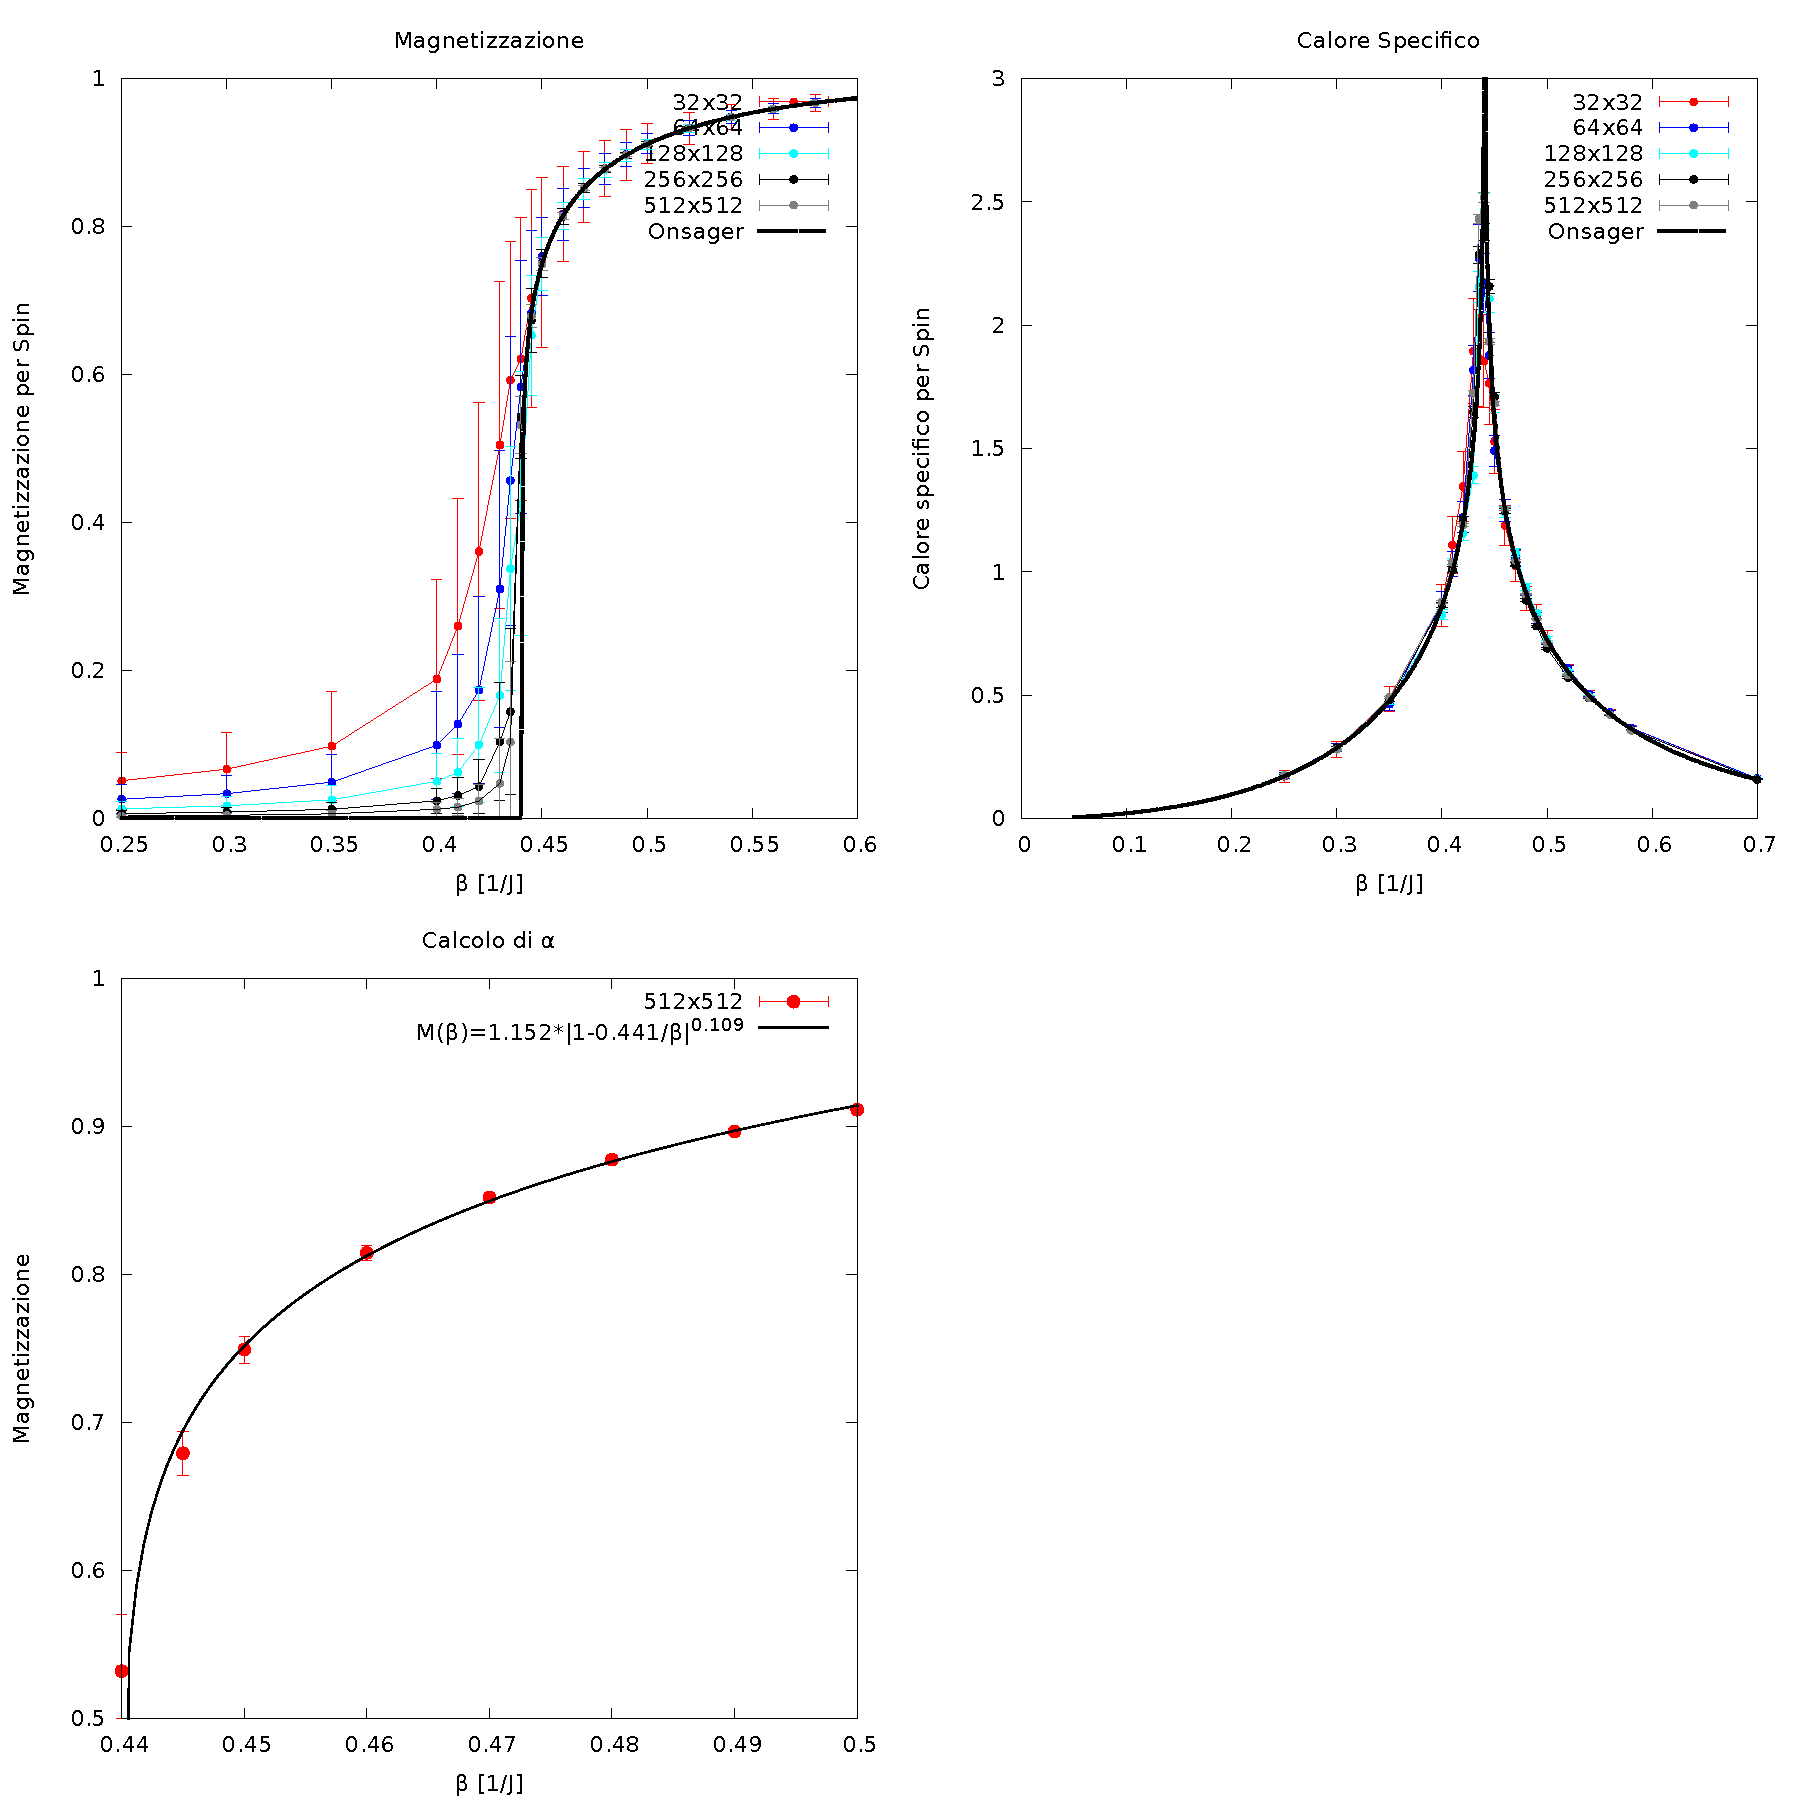
\includegraphics[width=120mm,angle=0,clip=]{../CPU/Result/Ising_Mag_Cv.pdf}
	\caption{Dati CPU}
	\label{figura:CPU}
\end{figure}

\begin{figure}
	\centering
	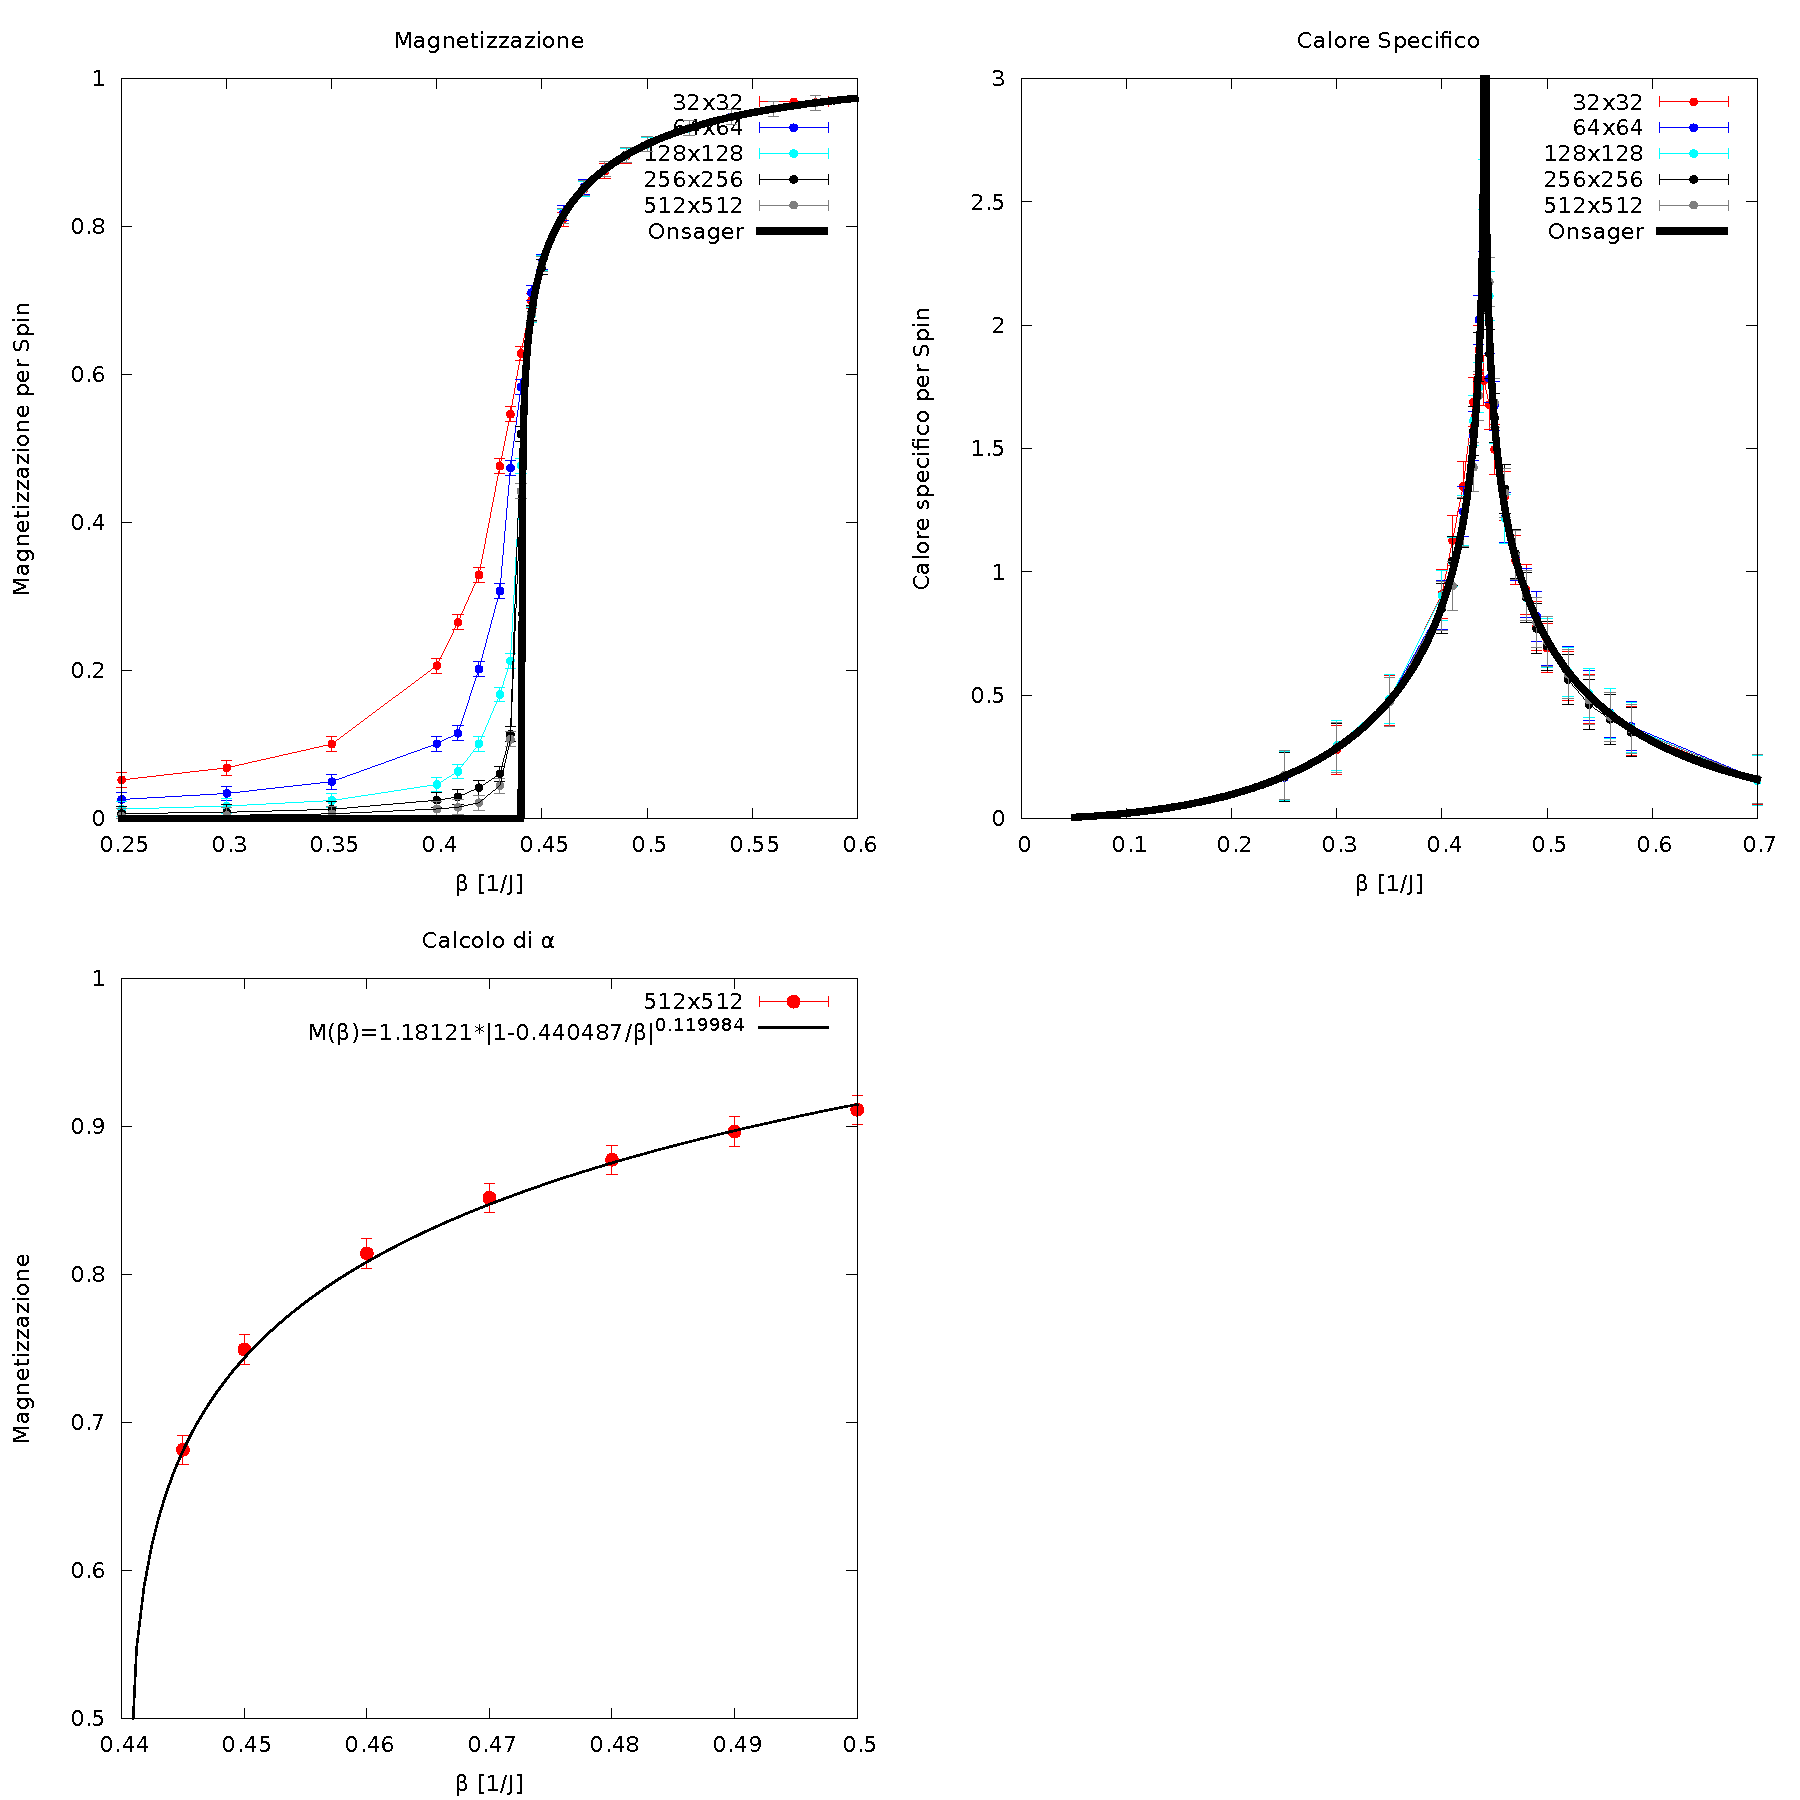
\includegraphics[width=120mm,angle=0,clip=]{../CUDA/Result/Res2/Ising_Mag_Cv.pdf}
	\caption{Dati GPU}
	\label{figura:GPU}
\end{figure}

\begin{figure}
	\centering
	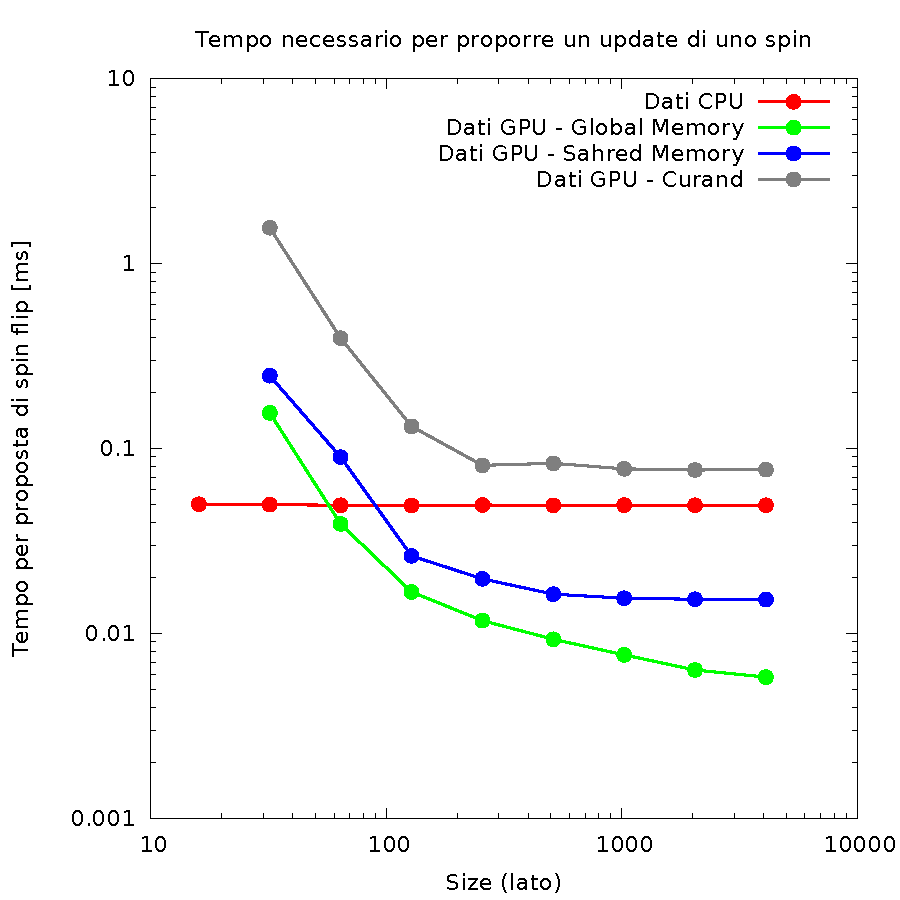
\includegraphics[width=120mm,angle=0,clip=]{../CPU-GPU-time.pdf}
	\caption{CPU/GPU}
	\label{figura:time}
\end{figure}








\end{document}
